\section{Data: Corpus-Monde v1}\label{sec:data}

\subsection{Sources and fusion}

The corpus fuses two public sources, each chosen for a different
epistemic role. \emph{CourtListener} (Free Law Project)
\citep{courtlistener} supplies the case universe: dockets, dates,
parties, opinion clusters, and oral-argument audio with transcripts,
harvested from the 2026-06-30 bulk release and cross-checked against
the REST API. The \emph{Supreme Court Database} (SCDB), 2025\_01
release, justice-centered case citation file \citep{spaeth2025},
supplies the ground truth: per-justice vote directions coded by a
single, long-running editorial team whose coding conventions are
public and whose known limitations are documented in the database
itself. CourtListener defines \emph{what happened procedurally};
SCDB defines \emph{what we count as a liberal or conservative vote}.

The corpus rule is deliberately narrow: every case argued before the
Court in the window from 1 October 2015 through 30 June 2024 (terms
OT2015 through OT2023) is included if it was argued and decided with
a full opinion. Per curiams, memorandum decisions, and cases decided
without argument are excluded---not because they are uninformative,
but because the prediction task is defined over argued cases whose
written record a model could read. Applying the rule yields 569
cases. Fusion keys on docket number with sub-docket-aware matching
(a nontrivial step: consolidated dockets appear in SCDB as
comma-separated lists and occasionally in variant forms such as
original-jurisdiction numbering), and every matched pair is checked
for term and case-name agreement.

\begin{table}[t]
\centering
\caption{Corpus-Monde v1 at a glance (frozen 2026-08-28).}
\label{tab:corpus}
\small
\begin{tabular}{@{}lr@{}}
\toprule
Quantity & Value \\
\midrule
Argued cases, OT2015--OT2023 & 569 \\
Justices appearing on the bench & 13 \\
Opinions (majority, dissent, concurrence) & 1{,}778 \\
Justice$\times$case votes, coded direction & 4{,}569 \\
Cases with SCDB vote coding & 96.1\% \\
Cases with oral-argument audio + transcript & 98.6\% \\
5--4 decisions & 79 \\
\quad of which sealed for the Final Test & 50 \\
Window & 2015-10-01 to 2024-06-30 \\
\bottomrule
\end{tabular}
\end{table}

\subsection{Freeze and provenance}

The corpus is frozen: the identity of the data is fixed by a rule,
and every artifact carries the hashes of everything upstream. The
SHA-256 of every raw source file (bulk archives, API pages, the SCDB
zip) is recorded at download time; the corpus build script
recomputes them before running; and the sealed-case list (below) is
itself committed as a SHA-256 of its JSON serialization. The intent
is that a skeptical reader can verify, without trusting the author,
that the data evaluated in Section~\ref{sec:results} is the data
described here---and that nothing was edited between the freeze and
the test.

Coverage statistics are reported with their failures rather than
their successes: 22 cases carry no SCDB match at all (mostly
original-jurisdiction and consolidated matters under variant
docketing), 27 additional cases match but have no coded issue area,
and audio coverage, while high (98.6\%), is absent for a handful of
late-window matters. These gaps flow through the pipeline as explicit
missing-value categories rather than silent deletions, and the vote
analysis of Section~\ref{sec:results} simply operates on the rows
where a coded direction exists (4{,}569 of an expected
4{,}730 vote slots).

\begin{figure}[t]
\centering
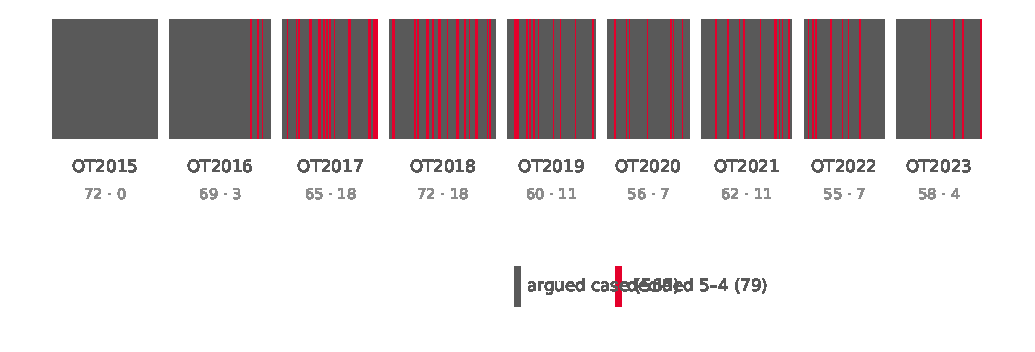
\includegraphics[width=\linewidth]{figures/fig1_corpus.pdf}
\caption{The corpus window. Each tick is one argued case, grouped by
term (counts below each group as argued~$\cdot$~5--4). Red ticks are
the 79 decisions that came down 5--4; the experiment's window is
deliberately the modern era of narrow majorities.}
\label{fig:corpus}
\end{figure}

\subsection{The bench}

Thirteen justices appear on the bench in the window, spanning three
natural cohorts: the five-justice block that opened the window
(Roberts, Scalia, Kennedy, Thomas, Ginsburg), the mid-window joiners
(Sotomayor, Kagan, Gorsuch, Kavanaugh, Barrett), and the closers
(Breyer's long service ending in 2021, Jackson arriving in 2022).
The 2020 death of Ginsburg and the two 2020 arrivals mean that no
single nine-member configuration spans the whole window; vote-level
analyses therefore condition on the justices actually sitting, and
pairwise agreement (Section~\ref{sec:results}) is computed on common
cases only, keeping the 60 pairs with at least 50 shared votes. Scalia
sits for only ten coded votes (he died in February 2016) and is
excluded from the pairwise matrix by the $n \ge 50$ rule---retained
everywhere else with his small-sample intervals displayed honestly.
